% !TEX root = seminararbeit.tex

\section{Basics and Related Work}
\label{basics-and-related-work}

\subsection{Scene-Graph}\label{scene-graph}

Scene-graphs can be used to group and organize \gls{3D} objects, their properties and
concerning transformations. A gls{DAG} can be used to represent a scene-graph.
It starts with a root node that is associated with one or more children. Each
child can be an object or a group, again containing more children. A group can
contain associated transformation information, like \emph{translation},
\emph{rotation} or \emph{scaling}. This structure has certain advantages
compared to applying all transformations to the raw meshes and sending
everything to the \gls{GPU}. \cite{realityprime} \gls{SSIML} \cite{Lenk:2012:MID:2338714.2338742} scene-graphs differ from the
above definition and there are three types of nodes:

\begin{itemize*}
  \item Transform nodes,
  \item geometry nodes and
  \item group nodes.
\end{itemize*}

\subsubsection{Culling}\label{culling}

Before using structures like scene-graphs, all polygons would be sent to
the \gls{GPU} and the \gls{GPU} would need to test which polygons are actually in the
view and thus need to be rendered. The problem of this approach is
that this information was only known after doing a lot of calculations
for every polygon already.\\
With a scene-graph it is possible to start from the root and traverse the
graph, testing the bounding box of each group and only sending it to the
\gls{GPU} if it is completely visible. If it is not, the whole sub-tree is not
sent to the \gls{GPU}. If it is partially visible the same process is applied
to the sub-tree.\\
By using a structure that retains more information about what it
represents it is possible to let the CPU do more of the heavy
lifting and unburden the \gls{GPU}.

\begin{quote}
  Rather than do the heavy work at the \gls{OpenGL} and polygon level,
  scene-graph architects realized they could better perform culling at
  higher level abstractions for greater efficiency. If we can remove the
  invisible objects first, then we make the hardware do less work and
  generally improve performance and the all-important frame-rate. \cite{realityprime}
\end{quote}

\subsubsection{Transformations}\label{transformations}

Another advantage is the way transformations work. Instead of applying
them to the meshes directly, and keeping track of what meshes belong to
the same object (like the chassis, the tires and the windows of a
car), they can simply be nested under the same transformation group. The
transformation thus applies to all objects associated with that group.

\subsubsection{Reuse}\label{reuse}

With the ability to address nodes it is possible to reuse their
information. If you have a car, it would be enough to have only one node
containing the geometry for a tire, all other tires are merely addressing
the tire with the geometry information (see listing \ref{list:defuse}).
That way the memory footprint of an application can be reduced.

\begin{listing}
  \begin{minted}[breaklines,bgcolor=bg]{html}
<Group>
  <Transform>
    <Shape def="chassis">
        <Appearance>
            <Material></Material>
        </Appearance>
        <Box></Box>
    </Shape>
  </Transform>
  <Transform>
    <Shape def="tire">
        <Appearance>
             <Material></Material>
        </Appearance>
        <Torus></Torus>
    </Shape>
  </Transform>
  <Transform>
    <Shape use="tire"/>
  </Transform>
  <Transform>
    <Shape use="tire"/>
  </Transform>
  <Transform>
    <Shape use="tire"/>
  </Transform>
</Group>
  \end{minted}
  \caption{Example \gls{X3D} group showing the use of \texttt{def} and \texttt{use}.}
  \label{list:defuse}
\end{listing}


\subsection{X3D}
\label{x3d} \gls{X3D} \cite{x3d} is the \gls{XML} representation of \gls{VRML} which was designed as a
universal interactive \gls{3D} exchange format, much like \gls{HTML} is for written
documents or \gls{SVG} for vector graphics. Due to its \gls{XML} structure it can be
integrated in \gls{HTML} documents, thus the Frauenhofer Institute pursued to
implement a runtime that could interpret and visualize \gls{X3D} in the browser, by
using a \gls{WebGL} context. It is called x3dom \cite{x3dom} and it is extensively used
by SceGraToo, the tool that arose from this thesis.

\subsection{x3dom}
\label{par:x3dom}

As said in the previous section, x3dom was developed by the Frauenhofer
Institute to realize the vision that started \gls{VRML} in the first place: \emph{mark
up interactive \gls{3D} content for the web}. On the web there are two entirely
different approaches to describe the same thing:

\begin{itemize*}
  \item imperative
  \item declarative
\end{itemize*}

\begin{longtable}[c]{@{}lll@{}}
  \caption{The matrix in this table classifies x3dom together with other common web technologies \cite{x3dom}.\label{tab:feature_matrix}}\\
  \toprule
  & 2D & \gls{3D} \tabularnewline
  \midrule
  \endhead
  Declarative & \gls{SVG} \cite{svg} & x3dom \cite{x3dom} \tabularnewline
  Imperative  & Canvas \cite{canvas} & \gls{WebGL} \cite{webgl} \tabularnewline
  \bottomrule
\end{longtable}

As can be seen in table \ref{tab:feature_matrix} x3dom complements the already existing technologies
perfectly.

\clearpage
\subsection{SSIML}
\label{ssiml}

Heterogeneous developer groups, groups that are comprised of people from
different backgrounds (programmers, \gls{3D} designers) have their difficulties
working together. They work in different domains and use different tools
adjusted to that domain. \cite{Glinz:2015:SUS:2802768.2802838}

SSIML is a graphical approach to unify the scene-graph model and the the
application model, thus making the communication between the different
parties easier.

It also serves as a code generation template.

\begin{figure}
  \centering
  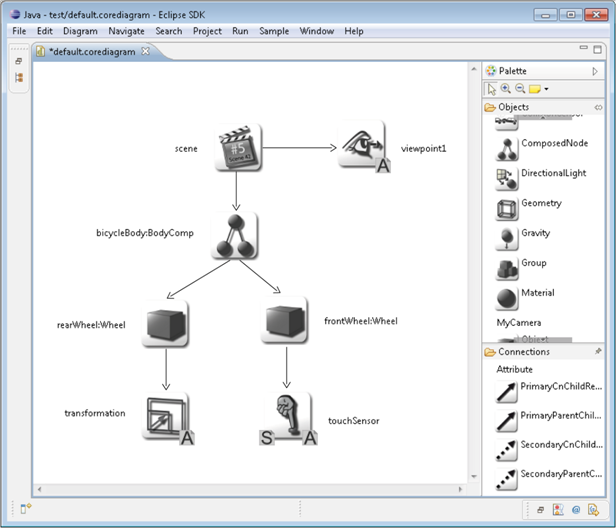
\includegraphics[width=12cm]{../assets/SSIML.png}
	\caption{This figure shows the graphical editor for SSIML. In particular it shows a scene comprising a bike. \cite{roundtrip3dwebsite}}
	\label{fig:ssimldiagram}
\end{figure}

\subsection{Roundtrip 3D}\label{roundtrip-3d}

As stated above, when developing \gls{3D} applications, many different
developers are involved, i.e.~\gls{3D} designers, programmers and, ideally,
also software designers (see figure \ref{fig:ssimldiagram}).

% TODO: convert to pdf
% 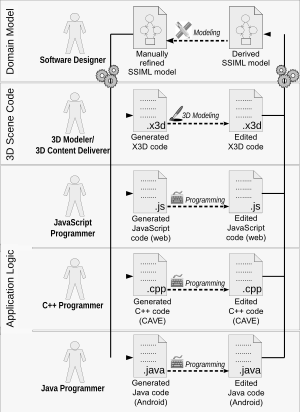
\includegraphics{../assets/csrd2014.svg}\\
% Roundtrip3D proposed process
% \href{http://dx.doi.org/10.1007/s00450-014-0258-8}{JLV15}

Roundtrip3D was a research project that, amongst others, resulted in a
graphical editor for \hyperref[ssiml]{SSIML} models. It offers an
approach for merging a developer's changes back into the main model.
After all working copies are merged back into the main model (dropping
unwanted or conflicting changes), all working copies are regenerated and
delivered to the individual developers. After each roundtrip every
developer has a copy of the project that is consistent with everyone
else's.

\subsection{Related Work}
\label{related-work}

The next section examines efforts and applications in the field of

\begin{itemize*}
  \item collaborative remote working on \gls{3D} models and
  \item online \gls{3D} editors.
\end{itemize*}

\subsubsection{3D Meteor}
\label{d-meteor0}

\begin{figure}[htbp]
  \centering
  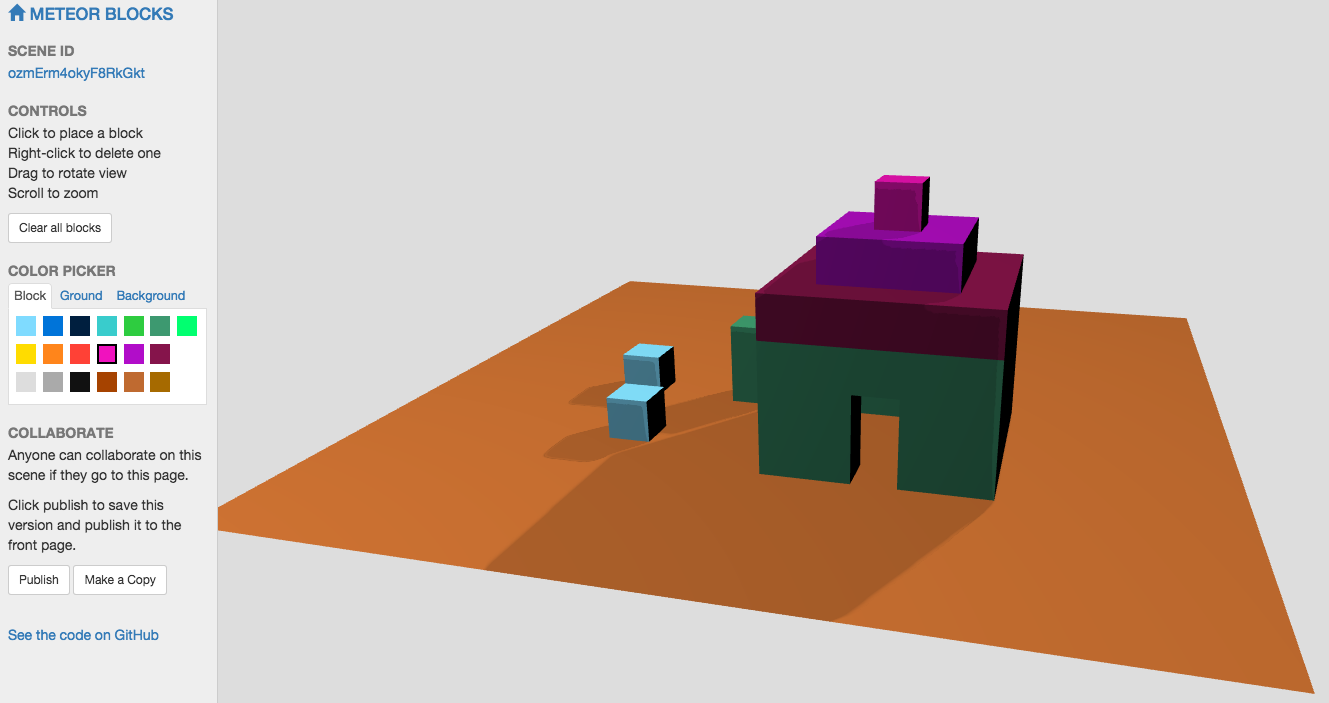
\includegraphics[width=12cm]{../assets/3dmeteor.png}
  \caption{This is a scene in 3dmeteor showing a house and a garden of cubes.}
	\label{fig:3dmeteor}
\end{figure}

This simple \gls{3D} editor allows the user to add and remove colored blocks to a
scene. The synchronization is leveraging meteor's database collection
subscription features. Meteor applications are comprised of a client side and a
server side. The client can subscribe to database collections and gets
automatically notified of changes to that collection by the server. The only
thing that actually is synchronized is an array of \emph{boxes}. A box is an
object with an x, y and z property describing its position. When a box is
added to the collection the collection is synchronized with the server. The
server informs all other browser instances that show this scene of the new box.
These browser instances reevalute the template that renders the x3dom scene to
the \gls{DOM} and the the \gls{DOM} is updated to contain the new box, thus synchronizing
the scene with the browser instance. \cite{3dmeteor}

\subsubsection{Blender Plugin}
\label{blender-plugin}

As part of an asset management system the Université du Québec à
Montréal implemented a plugin for Blender for collaborative working. An
artist can record changes to wiremeshes and store them on a server.
Another artist can download these changes and apply them to his working
copy. The change sets are a simple list of vertices and their movement in the
x, y and z space (see listing \ref{blenderplugin}). \cite{LCR07}

\begin{listing}
  \begin{minted}[breaklines,bgcolor=bg]{text}
95 [0.0000, 0.0000, 0.0000]
295 [0.0027, 0.0013, 0.0000]
309 [0.2123, 0.1001, 0.0000]
311 [0.3029, 0.1429, 0.0000]
  \end{minted}
  \caption{This shows a change set of 4 polygons and how they where moved.}
  \label{blenderplugin}
\end{listing}

These are saved on the server and another user working on the same
object can apply them to his working copy. They can actually be applied
to any object that has the same number of vertices. That is also a
shortcoming. Adding or removing vertices cannot be handled by the
plugin. It is also not in real time, so it is more comparable to version
control system like \gls{git} just for \gls{3D} models.

\subsubsection{Gizmos}\label{gizmos}

Gizmos, also called manipulators, are handles or bounding boxes with
handles that manipulate their containing objects in a predefined way when
dragged. \cite{wikigizmo}

In \gls{X3D} gizmos can be realized with specialized X3DDragSensorNodes \cite{x3ddragsensornode}, like:

\begin{description*}
\item[SphereSensor]
  SphereSensor converts pointing device motion into a spherical rotation around the origin of the local coordinate system. \cite{spheresensor}
\item[CylinderSensor]
  The CylinderSensor node converts pointer motion (for example, from a mouse) into rotation values, using an invisible cylinder of infinite height, aligned with local Y-axis. \cite{cylindersensor}
\item[PlaneSensor]
  PlaneSensor converts pointing device motion into 2D translation, parallel to the local Z=0 plane. Hint: You can constrain translation output to one axis by setting the respective minPosition and maxPosition members to equal values for that axis. \cite{planesensor}
\end{description*}

The sensors track drag events on their siblings. In the example in figure
\ref{fig:x3dgizmo} (which is taken directly from the x3dom website) the
PlaneSensor tracks drag events on the cones and the cylinder that make up the
cyan handle. Part of the structure of the scene can be seen in listing
\ref{planesensor}.

Every time it detects a drag event it converts it into a 2D
transformation and raises an \texttt{onOutPutChange} event.\\
The callback \texttt{processTranslationGizmoEvent} is registered as an event handler.
In this function the position of the handle is adjusted to make it
follow the drag movement, also the position of the teapot is adjusted.

Having the handles being \gls{3D} objects within the scene, that look
touchable and intractable, make it easier for users find their way
around the application. Instead of having to learn keyboard shortcuts
users simply use their intuition and knowledge about how to interact with
objects in the real world.

The pictures in \ref{blender} to \ref{fig:x3dgizmo} show different gizmos from
different applications.

\begin{listing}
  \begin{minted}[breaklines,bgcolor=bg]{html}
<group>
  <planeSensor autoOffset='true' axisRotation='1 0 0 -1.57' minPosition='-6 0' maxPosition='6 0' onoutputchange='processTranslationGizmoEvent(event)'>
  </planeSensor>

  <transform id='translationHandleTransform'>
    <transform translation='0 -5.5 8' rotation='0 1 0 1.57'>
      <transform translation='0 0 1.5' rotation='1 0 0 1.57'>
        <shape DEF='CONE_CAP'>
          <appearance DEF='CYAN_MAT'><material diffuseColor='0 1 1'></material></appearance>
          <cone height='1'></cone>
        </shape>
      </transform>
      <transform rotation='1 0 0 -1.57'>
        <shape>
          <appearance USE='CYAN_MAT'></appearance>
          <cylinder></cylinder>
        </shape>
      </transform>
      <transform translation='0 0 -1.5' rotation='1 0 0 -1.57'>
        <shape USE='CONE_CAP'></shape>
      </transform>
    </transform>
  </transform>
</group>
  \end{minted}
  \caption{This shows a group containing a planeSensor. It shows a part of the scene depicted in figure \ref{fig:x3dgizmo}.}
  \label{planesensor}
\end{listing}

\begin{figure}[htbp]
  \begin{minipage}{.5\textwidth}
    \centering
    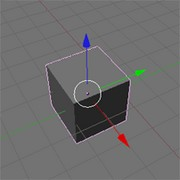
\includegraphics[width=0.9\textwidth]{../assets/Manual-Manipulators-Translate.jpg}\\
  	a) A translation gizmo. \cite{blenderwiki}
  \end{minipage}
  \begin{minipage}{.5\textwidth}
    \centering
    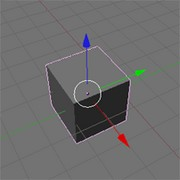
\includegraphics[width=0.9\textwidth]{../assets/Manual-Manipulators-Translate.jpg}\\
  	b) Rotation gizmo. \cite{blenderwiki}
  \end{minipage}\\
  \begin{minipage}{.5\textwidth}
    \centering
    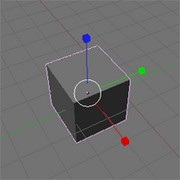
\includegraphics[width=0.9\textwidth]{../assets/Manual-Manipulators-Scale.jpg}\\
  	c) Scale gizmo. \cite{blenderwiki}
  \end{minipage}
  \begin{minipage}{.5\textwidth}
    \centering
    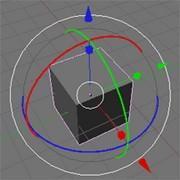
\includegraphics[width=0.9\textwidth]{../assets/Manual-Manipulators-Combo.jpg}\\
  	d) All gizmos together. \cite{blenderwiki}
  \end{minipage}
  \caption{The same cube in Blender with different gizmos/transformers enabled.}
  \label{blender}
\end{figure}
\begin{figure}[]
  \centering
  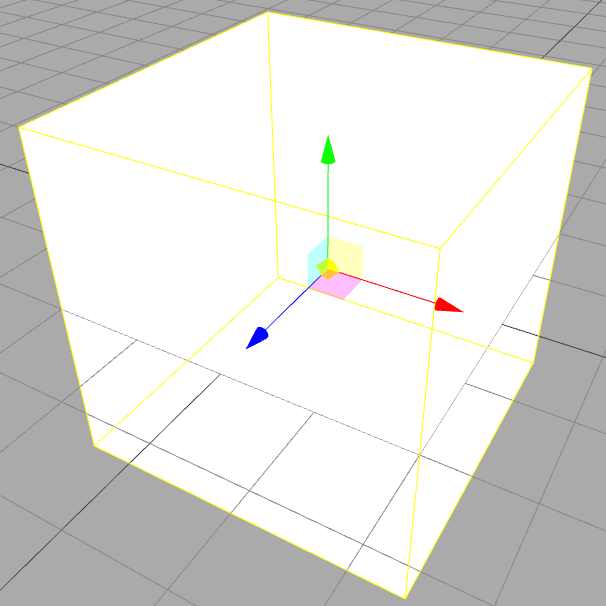
\includegraphics[width=12cm]{../assets/threejs-editor.png}
	\caption{ Shows translate gizmos along the x, y and z axis as well as gizmos that translate the cube along the xy, xz, yz and frustum plane. \cite{threejseditor} }
\end{figure}
\begin{figure}[]
  \centering
  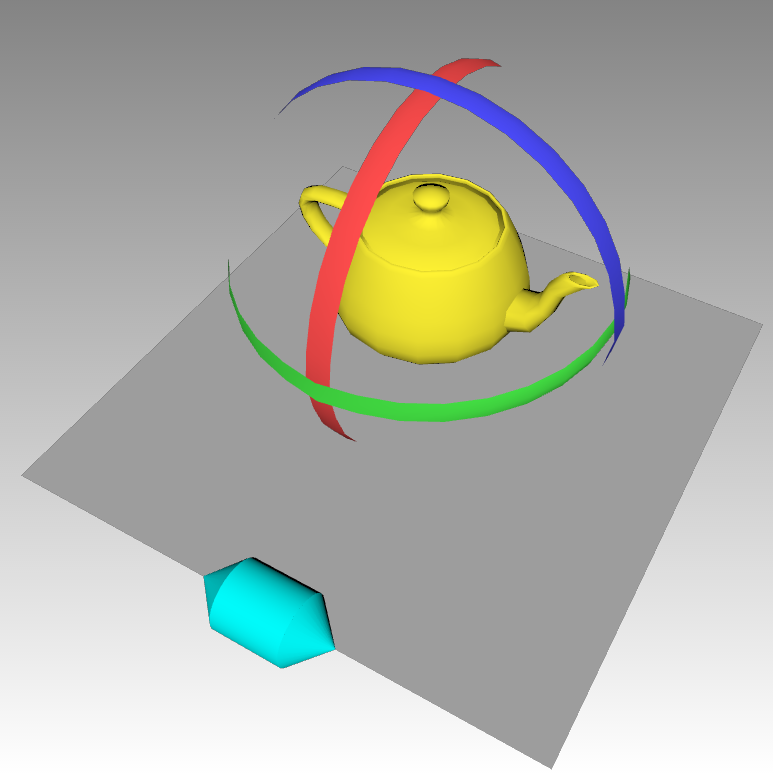
\includegraphics[width=12cm]{../assets/x3dom-gizmo-example.png}
	\caption{ Shows an official x3dom tutorial for using sensors to create gizmos. \cite{x3dgizmo} }
	\label{fig:x3dgizmo}
\end{figure}

\clearpage

\subsubsection{Component Editor}
\label{component-editor30}

On the 12th of June 2015 the x3dom maintainers released their Component Editor. \cite{componenteditor}
It was released after the the work on \gls{Roundtrip3D} started.
Its development took about a year and three people working part-time on it. \cite{componenteditoreffort}
Although it does offer all the wanted scene composition features, it lacks the ability to:

\begin{itemize*}
  \item Load an existing \gls{X3D} file,
  \item save the scene as an \gls{X3D} file and
  \item upload \gls{X3D} files that can be included as inlines.
\end{itemize*}

Scenes can only be loaded and saved as a \gls{JSON} representation (see listing~\ref{componenteditorjson}).
Conversion between the formats may be possible, but meta information like \gls{ID}s in comments would be lost.

\begin{listing}
  \begin{minted}[breaklines,bgcolor=bg]{json}
{
  "0": {
    "type": "Box",
    "transform": "1.000000, 0.000000, 0.000000, 0.000000, \n0.000000, 1.000000, 0.000000, 0.000000, \n0.000000, 0.000000, 1.000000, 0.000000, \n0.000000, 0.000000, 0.000000, 1.000000",
    "referencePoints": ["p1", "p2", "p3", "p4", "p5", "p6"],
    "parameters": {
      "Size": [1, 1, 1],
      "Positive Element": "true"
    }
  }
}
  \end{minted}
  \caption{The \gls{JSON} format used by the component editor to save scenes.}
  \label{componenteditorjson}
\end{listing}

\subsubsection{Real-Time Collaborative Scientific WebGL Visualization with Web Sockets}
\label{rtcswvwws}

Using web sockets instead of AJAX is an interesting approach.
\cite{Marion:2012:RCS:2338714.2338721} Especially the cut down on latency. It is
over all very similar to the approach that was considered for SceGraToo, but not
implemented due to time constraints. In the end the differences between
SceGraToo's requirements and theirs outweigh the similarities. \gls{Roundtrip3D} not only
has to visualize a scene, but also manipulate it. And to achieve a spector mode
like in this work not only the viewpoint would have to be synchronized but also
the whole scene. This can either be done by sending the whole scene to the other
clients on every change, or sending change sets, which poses an interesting
challenge. They visualize a specific dataset in a threejs's specific \gls{JSON} format
\cite{threejs-format}. \gls{Roundtrip3D} only needs to render \gls{X3D} scenes, converting the
scene into another format and have it rendered by another scene graph framework
is unnesesary, since x3dom does a pretty good job doing this.

\subsubsection{ParaViewWeb}
\label{paraviewweb-pvweb}

Simple to use out of the box, but needs a paraview server instance and
paraview does not support \gls{X3D} as an input format. So using this is unfortunately
not possible unless an import filter is written. The visualization is
mainly meant to explore data sets. There is no easy way to manipulate
the input data. This can only happen by extending the visualization
pipeline via python scripts on the server.
